\documentclass[12pt]{article}  
\usepackage[boxruled,lined]{algorithm2e} \usepackage{booktabs}
\usepackage{amsmath} \usepackage{amsthm} \usepackage{amsfonts} 
\usepackage{xparse} \usepackage{bbm} \usepackage{color,soul} \usepackage{framed} \usepackage[margin=0.5in]{geometry} \usepackage{hyperref} \usepackage{mathtools}
\usepackage{multicol}
\usepackage[dvipsnames]{xcolor}
\usepackage{tikz}
\usepackage{pgfplots}  
\usetikzlibrary{positioning}
\usetikzlibrary{calc}

\newtheorem{theorem}{Theorem}[section] \newtheorem{lemma}[theorem]{Lemma} \newtheorem{proposition}[theorem]{Proposition} \newtheorem{corollary}[theorem]{Corollary}  \DeclarePairedDelimiter{\ceil}{\lceil}{\rceil} \DeclarePairedDelimiter{\floor}{\lfloor}{\rfloor} \DeclareMathOperator*{\argmin}{arg\,min} \DeclareMathOperator*{\argmax}{arg\,max} \newcommand{\D}{\mathrm{d}} \SetKwInput{KwInput}{Input} \SetKwInput{KwOutput}{Output}  \begin{document}
\renewcommand{\d}[1]{\ensuremath{\operatorname{d}\!{#1}}}

\section{Logistic Regression}\vspace{.1pt} \hrule height 2pt \smallskip \renewcommand{\arraystretch}{1}% Tighter \begin{description} \item[Intro] 
This model assumes that the log odds-ratio can be fit by a linear model. We start with the probability mass function for a \href{https://en.wikipedia.org/wiki/Bernoulli_distribution}{Bernoulli trial}: $f(y;p) = p^y \times (1-p)^{(1-y)}$ for $y \in \{0, 1\}$. We are interested in estimating what $p$ is, and so it's natural to conceive of a maximum likelihood estimator; since $\log$ monotone we can apply this transformation without changing the maximizer. The log-likelihood is given by $y \log p + (1-y) \log (1-p)$ using \href{https://en.wikipedia.org/wiki/Logarithm#Logarithmic_identities}{properties of logarithms}. In optimization, we generally work to minimize objective functions, and so it's then natural to set our (objective) \emph{loss function}
to be $- \left[y \log p + (1-y) \log (1-p)\right]$. In summary, we 
have, for $\sigma(x) = \frac{1}{1 + \exp(-x)}$:
\begin{align}
  z &= w^Tx + b \\
  \hat y &= a = \sigma(z) \\
  \mathcal{L}(a, y) &= - \left[y \log (a) + (1-y) \log (1-a)\right] \end{align}

We can draw a \emph{computation graph} to describe the forward pass as follows:
\begin{center}
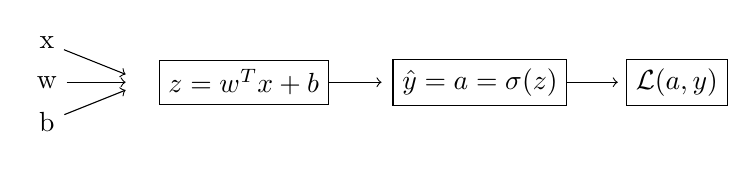
\begin{tikzpicture}
  \node (x) at (0, 1) {x};
  \node (w) at (0,.5) {w};
  \node (b) at (0, 0) {b};
  \draw[->] (x) to (1, .6);
  \draw[->] (w) to (1, .5);
  \draw[->] (b) to (1, .4);
  \node[draw=black,rectangle] (z) at (2.5, .5) {$z = w^Tx + b$};
  \draw[->] (z) to (4.25, .5);
  \node[draw=black,rectangle] (yhat) at (5.5, .5) {$\hat y = a = \sigma(z)$};
  \draw[->] (yhat) to (7.25, .5);
  \node[draw=black,rectangle] (loss) at (8, .5) {$\mathcal L (a,y)$};
\end{tikzpicture}
\end{center} We seek to learn $w, b$ to minimize the loss function. \emph{Back propogation} proceeds as follows:

{
\small{
\begin{align*}
\texttt{da} &= \frac{\partial \mathcal L}{\partial a} = - \left(\frac{y}{a} - \frac{1-y}{1-a}\right) = \frac{-y}{a} + \frac{1-y}{1-a}. \\
  \texttt{dz} &= \frac{\partial \mathcal L}{\partial z} = \frac{\partial \mathcal L}{\partial a}\frac{\partial a}{\partial z} = \left(\frac{-y}{a} + \frac{1-y}{1-a}\right) \times a(1-a) = \frac{-y}{a} \cdot a(1-a) + \frac{1-y}{1-a} \cdot (1-a) a = -y(1-a)+ (1-y)a \\ &= ay - y + a - ay = a - y.  \\
\texttt{dw} &= \frac{\partial \mathcal L}{\partial w} \overset{?}{=} \frac{\partial \mathcal L}{\partial z} \frac{\partial z}{\partial w} = (a-y) x^T. \\
\texttt{db} &= \frac{\partial \mathcal L}{\partial b} = \frac{\partial \mathcal L}{\partial z} \underbrace{\frac{\partial z}{\partial b}}_{=1}. \end{align*}
}
}
Our update rule then becomes: $w := w - \alpha \texttt{dw}$, and $b := b - \alpha \texttt{db}$. Our (average) \emph{cost} function is defined as $J(w,b) = \frac{1}{m} \sum_{i=1}^m \mathcal L(a^{(i)}, y^{(i)})$. Since $\frac{\partial}{\partial \cdot}$ is a linear operator, obtaining gradients is quite straightforward since we are left with a series of derivatives of loss functions, which we calculated above.
\begin{align*}    \frac{\partial J}{\partial w} = \frac{1}{m} \sum \frac{\partial \mathcal L}{\partial w}, \hspace{15pt} \textrm{and} \hspace{15pt} \frac{\partial J}{\partial b} = \frac{1}{m} \sum \frac{\partial \mathcal L}{\partial b} \end{align*}
Our optimization routine then can be written as in algorithm \ref{alg: logisticreg}

{\small
\begin{algorithm}[H]
  \label{alg: logisticreg}
  \caption{Logistic Regression - Optimization}   \For{\texttt{i in range(m)}} {
    $z^{(i)} = w^Tx^{(i)} + b$ \\
    $a^{(i)} = \sigma(z^{(i)})$ \\
    $J += - \left[ y^{(i)} \log a^{(i)} + (1-y^{(i)}) \log (1 - a^{(i)}) \right]$ \\
    $\partial d z^{(i)} = a^{(i)} - y^{(i)}$ \\
    $\partial d w += \partial d z^{(i)} {x^{(i)}}^T$ \\
    $\partial d b += \partial d z^{(i)}$
}
$J /= m$ \\
$\partial w /= m$ \\
$\partial b /= m$ \end{algorithm}
}
The above concludes one round of \href{https://en.wikipedia.org/wiki/Gradient_descent}{Gradient Descent}. We repeat this procedure many times until training loss (and ideally test loss ) is sufficiently minimized. We remark that it's possible to remove both \texttt{for} loops (over the training data, and over the parameters in $w$) by using vectorized operations in \texttt{numpy}. We execute this in code \href{https://github.com/asantucci/NN/blob/master/logistic_regression.py#L46}{here}.

\section{Neural Networks with 2-layers}
\vspace{-10pt}
We previously saw a simple computation graph. 
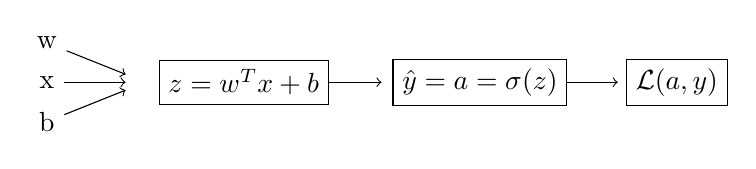
\begin{tikzpicture}   \node (w) at (0, 1) {w};
  \node (x) at (0, .5) {x};
  \node (b) at (0,0) {b};
  \draw[->] (x) to (1, .5);
  \draw[->] (w) to (1, .6);
  \draw[->] (b) to (1, .4);
  \node[draw=black,rectangle] (z) at (2.5, .5) {$z = w^Tx + b$};
  \draw[->] (z) to (4.25, .5);
  \node[draw=black,rectangle] (yhat) at (5.5, .5) {$\hat y = a = \sigma(z)$};
  \draw[->] (yhat) to (7.25, .5);
  \node[draw=black,rectangle] (loss) at (8, .5) {$\mathcal L (a,y)$};
\end{tikzpicture}
\subsection{Understanding Small Neural Networks}
A Neural Network can be constructed by stacking together sigmoids, depicted as follows:
\begin{figure}[h]
\centering
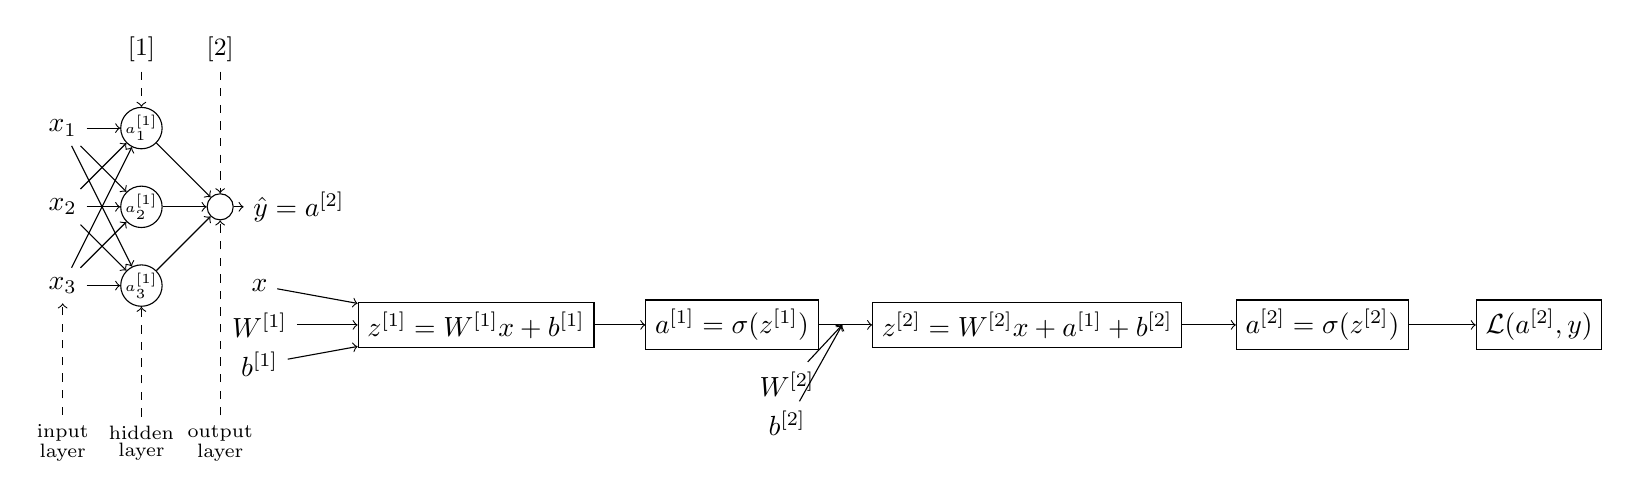
\begin{tikzpicture}
  \node (x1) at (0, 1) {$x_1$};
  \node (x2) at (0, 0) {$x_2$};
  \node (x3) at (0,-1) {$x_3$};
  \node (inputlayer) at (0, -3) {$\substack{\textrm{input}\\ \textrm{layer}}$};
  \draw[->,dashed] (inputlayer) to (x3);
  \node (lbl) at (1,2) {\small{$[1]$}}; 
  \node[draw=black,circle,inner sep = 0pt] (n1) at (1, 1) {\tiny $a_1^{[1]}$};
  \draw[->,dashed] (lbl) to (n1);
  \node[draw=black,circle,inner sep = 0pt] (n2) at (1, 0) {\tiny $a_2^{[1]}$};
  \node[draw=black,circle,inner sep = 0pt] (n3) at (1,-1) {\tiny $a_3^{[1]}$};
  \node (hiddenlayer) at (1, -3) {$\substack{\textrm{hidden}\\ \textrm{layer}}$};
  \draw[->,dashed] (hiddenlayer) to (n3);
  \draw[->] (x1) to (n1);
  \draw[->] (x1) to (n2);
  \draw[->] (x1) to (n3);   \draw[->] (x2) to (n1);
  \draw[->] (x2) to (n2);
  \draw[->] (x2) to (n3);   
  \draw[->] (x3) to (n1);
  \draw[->] (x3) to (n2);
  \draw[->] (x3) to (n3); 
  \node[draw=black,circle] (m1) at (2,0) {};
  \node (lbl2) at (2,2) {\small{$[2]$}}; 
  \draw[->,dashed] (lbl2) to (m1);
  \node (yhat) at (3,0) {$\hat y = a^{[2]}$};
  \node (outputlayer) at (2, -3) {$\substack{\textrm{output}  \\ \textrm{layer}}$};
  \draw[->,dashed] (outputlayer) to (m1);
  \draw[->] (n1) to (m1);
  \draw[->] (n2) to (m1);
  \draw[->] (n3) to (m1);
  \draw[->] (m1) to (yhat);
  \node (x) at (2.5, -1) {$x$};
  \node (w1) at (2.5, -1.5) {$W^{[1]}$};
  \node (b1) at (2.5, -2) {$b^{[1]}$};
  \node[draw=black,rectangle] (z1) at (5.25, -1.5) {$z^{[1]} = W^{[1]}x + b^{[1]}$};
  \draw[->] (x) to (z1);
  \draw[->] (w1) to (z1);
  \draw[->] (b1) to (z1);
  \node[draw=black,rectangle] (a1) at (8.5, -1.5) {$a^{[1]} = \sigma (z^{[1]})$};
  \draw[->] (z1) to (a1);
  \node[draw=black,rectangle] (z2) at (12.25, -1.5) {$z^{[2]} = W^{[2]}x + a^{[1]} + b^{[2]}$};
  \draw[->] (a1) to (z2);
  \node (w2) at (9.2, -2.25) {$W^{[2]}$};
  \node (b2) at (9.2, -2.75) {$b^{[2]}$};
  \draw[->] (w2) to (9.9, -1.5);
  \draw[->] (b2) to (9.9, -1.5);
  \node[draw=black,rectangle] (a2) at (16, -1.5) {$a^{[2]} = \sigma(z^{[2]})$};
  \draw[->] (z2) to (a2);
  \node[draw=black,rectangle] (l) at (18.75, -1.5) {$\mathcal L(a^{[2]},y)$};
  \draw[->] (a2) to (l);
\end{tikzpicture}
\caption{A 2-layer Neural Network (you could say we don't count the input layer, or you could say we do but we index starting from zero).}
\end{figure}
\newline
\vspace{-40pt}
\paragraph{Terminology and Notation}
Each \emph{neuron} in the graph consists of both a linear transformation and a non-linear activation function, i.e. the first stack of nodes will produce a $z$ and an $a$. We use the super-script square brackets $[\hspace{2pt} ]$ to denote a stack of nodes, i.e. a layer, not to be confused with super-script parentheses which index training examples. I.e. $a^{[\ell]}_i$ denotes the output of an activation function in layer $\ell$ for the $i$th neuron.
The key difference between our Logistic Regression and 
this (or any) Neural Network is that we simply repeat linear transformations followed by non-linear activation functions \emph{multiple times}.
The reason why we call the intermediary layer a ``hidden'' layer is because we do not observe what these values are to be in the training set. By convention, we define  $a^{[0]} = X$. We can further refer to the hidden layer by ${a^{[1]}} = \begin{bmatrix}   a_1^{[1]} & a_2^{[1]} & a_3^{[1]}  \end{bmatrix}^T$. Notice that the hidden layer and output layer have parameters $W^{[\cdot]}$ and $b^{[\cdot]}$ associated with them. 

\paragraph{Visualizing a Neuron}
Let's take a look at neural network representation in a bit more detail. We can think about each neuron as being divided into two parts: one which performs a linear transformation and another which performs an activation function. The mental model is:
\begin{figure}[h]
  \centering   
  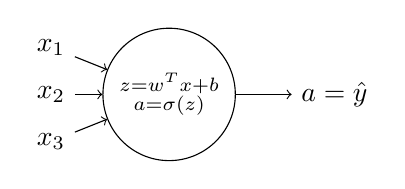
\begin{tikzpicture}[scale=0.6]     
    \node (x1) at (-1, 1) {$x_1$};
    \node (x2) at (-1, 0) {$x_2$};
    \node (x3) at (-1,-1) {$x_3$};
    \node[draw,circle] (neuron) at (1.5,0) {$\substack{z = w^Tx + b \\ a = \sigma(z)}$};
    \draw[->] (x1) to (neuron);
    \draw[->] (x2) to (neuron);
    \draw[->] (x3) to (neuron);
    \node (output) at (5,0) {$a = \hat y$};
    \draw[->] (neuron) to (output);
  \end{tikzpicture} \end{figure}
\newline
In general, we'll have something as follows for the first neuron in the hidden layer, and to be crystal clear we draw out the second neuron as well.
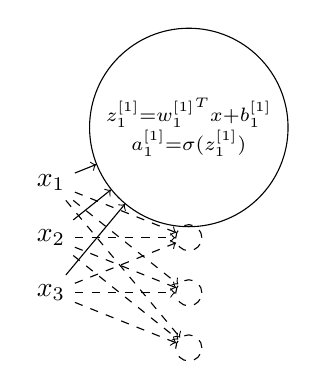
\begin{tikzpicture}[scale=0.7]     
  \node (x1) at (0, 1) {$x_1$};
    \node (x2) at (0, 0) {$x_2$};
    \node (x3) at (0,-1) {$x_3$};
    \node[draw,circle] (neuron) at (2.5,2) {$\substack{z_1^{[1]} = {w_1^{[1]}}^Tx + b_1^{[1]} \\ a_1^{[1]} = \sigma(z_1^{[1]})}$};
    \draw[->] (x1) to (neuron);
    \draw[->] (x2) to (neuron);
    \draw[->] (x3) to (neuron);
    \node[draw,circle,dashed] (n2) at (2.5,0 ) {};     \node[draw,circle,dashed] (n3) at (2.5,-1) {}; 
    \node[draw,circle,dashed] (n4) at (2.5,-2) {}; 
    \draw[->,dashed] (x1) to (n2);
    \draw[->,dashed] (x2) to (n2);
    \draw[->,dashed] (x3) to (n2);
    \draw[->,dashed] (x1) to (n3);
    \draw[->,dashed] (x2) to (n3);
    \draw[->,dashed] (x3) to (n3);
    \draw[->,dashed] (x1) to (n4);
    \draw[->,dashed] (x2) to (n4);
    \draw[->,dashed] (x3) to (n4);
\end{tikzpicture}
\hspace{20pt} 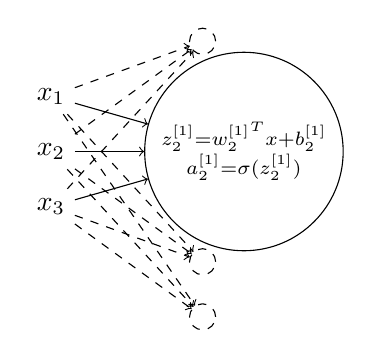
\begin{tikzpicture}[scale=0.7]     
    \node (x1) at (0, 1) {$x_1$};
    \node (x2) at (0, 0) {$x_2$};
    \node (x3) at (0,-1) {$x_3$};
    \node[draw,circle,dashed] (neuron) at (2.75,2) {};
    \draw[->,dashed] (x1) to (neuron);
    \draw[->,dashed] (x2) to (neuron);
    \draw[->,dashed] (x3) to (neuron);
    \node[draw,circle] (n2) at (3.5,0 ) {$\substack{z_2^{[1]} = {w_2^{[1]}}^Tx + b_2^{[1]} \\ a_2^{[1]} = \sigma(z_2^{[1]})}$};     
    \node[draw,circle,dashed] (n3) at (2.75,-2) {}; 
    \node[draw,circle,dashed] (n4) at (2.75,-3) {}; 
    \draw[->] (x1) to (n2);
    \draw[->] (x2) to (n2);
    \draw[->] (x3) to (n2);
    \draw[->,dashed] (x1) to (n3);
    \draw[->,dashed] (x2) to (n3);
    \draw[->,dashed] (x3) to (n3);
    \draw[->,dashed] (x1) to (n4);
    \draw[->,dashed] (x2) to (n4);
    \draw[->,dashed] (x3) to (n4);
\end{tikzpicture} 
To avoid having to calculate $z_i^{[\ell]}$ using a \texttt{for}
loop, we can instead use a matrix multiply, where $W^{[1]} \in \mathbb R^{n_1, n_x}$:
$$
W^{[1]}x + b^{[1]} = 
\underbrace{\begin{bmatrix}    & {w_1^{[1]}}^T & \\
   & {w_2^{[1]}}^T & \\    & {w_3^{[1]}}^T & \\    
   & {w_4^{[1]}}^T & \\ 
\end{bmatrix}}_{\in \mathbb R^{4, 3}} \begin{bmatrix} x_1 \\ x_2 \\ x_3  \end{bmatrix} + \begin{bmatrix}   b_1^{[1]} \\ b_2^{[1]} \\ b_3^{[1]} \\ b_4^{[1]} \end{bmatrix} = \begin{bmatrix}   z_1^{[1]} \\
  z_2^{[1]} \\
  z_3^{[1]} \\
  z_4^{[1]} \\ \end{bmatrix} = z^{[1]}
$$
We can then write ${a^{[1]}}^T = \begin{bmatrix}   a_1^{[1]} & a_2^{[1]} & a_3^{[1]} & a_4^{[1]} \end{bmatrix} = \sigma (z^{[1]})$ where the $\sigma(\cdot)$ is applied element-wise.
Given an input $x$, we set $a^{[0]} = x$ and we compute forward steps: $z^{[\ell]} = W^{[\ell]}a^{[\ell-1]} + b^{[\ell]}$
for each layer in the network.

\paragraph{Vectorization} Suppose we have a single hidden-layer neural network. As per above, the forward propagation involves computing: 
$  z^{[1]} = W^{[1]}a^{[0]} + b^{[1]}; \hspace{10pt} a^{[1]} = \sigma(z^{[1]}); \hspace{10pt} 
   z^{[2]} = W^{[2]}a^{[1]} + b^{[2]}; \hspace{10pt} 
   a^{[2]} = \sigma(z^{[2]}).
$
We need to replicate this procedure for each of our $m$ training samples. I.e. we need to feed each training example through the network to get an output. Let our final output be denoted by $a^{[\ell](j)}$ denote the output for the activation function for the $j$th training example at the $\ell$th layer in our network. So in our case above, $a^{[2](j)}$ is the output for the $j$th training example.
We'd like to avoid applying a \texttt{for} loop over each of our $m$ training examples, like so:
{\footnotesize
\begin{algorithm}[h]
  \caption{Naive Forward Propagation on a 2-layer Neural Network}   \For{i = 1 to m}{
    $z^{[1](i)} = W^{[1]}x^{(i)} + b^{[1]}$ \\
    $a^{[1](i)} = \sigma(z^{[1]}(i))$ \\
    $z^{[2](i)} = W^{[2]}a^{[1](i)} + b^{[2]}$ \\
    $a^{[2](i)} = \sigma(z^{[2]}(i))$
  } \end{algorithm}
}
\newline
\vspace{-.5ex}Recall we arranged our input matrix such that each column is an observation, i.e. $X = \begin{bmatrix}    | & | & & | \\    x^{(1)} & x^{(2)} & \ldots & x^{(m)} \\   | & | & & |  \end{bmatrix} \in \mathbb R^{n_x, m}$. Then,
$  
  Z^{[1]} = W^{[1]} X + b^{[1]}; \hspace{10pt}
  A^{[1]} = \sigma(Z^{[1]}); \hspace{10pt}
  Z^{[2]} = W^{[2]} A^{[1]} + b^{[2]}; \hspace{10pt}
  A^{[2]} = \sigma(Z^{[2]})
$ To be explicit, $Z^{[1]}$ is also arranged with observations in columns, i.e. $Z^{[1]} = \begin{bmatrix}   | & | & & | \\ z^{[1](1)} & z^{[1](2)} & \ldots & z^{[1](m)} \\ | & | & & | \end{bmatrix}$ and $A^{[1]} = \begin{bmatrix}    | & | & & | \\    a^{[1](1)} & a^{[1](2)} & \ldots & a^{[1](m)}  \\  | & | & & | \end{bmatrix}$.\footnote{As one scans matrix $A^{[\ell]}$ from left to right, we scan through observations or training examples, and as we scan from top to bottom we scan through the activations of different hidden units.}

\subsection{Activation Functions}
\paragraph{Hyperbolic Tangent}
Another activation function to consider is $\tanh (z) = \frac{e^z - e^{-z}}{e^z + e^{-z}}$. It's a shifted and rescaled version of the sigmoid function, which ranges from $[-1, 1]$ and cross the $x$-axis at zero; it is intuitively thought to perform better than a sigmoid activation function since it has the effect of ``centering'' the data in the intermediate layers of the network around zero. The one exception is the output layer: if we are predicting binary classification it makes sense to use sigmoid since our target values are in $\{0, 1\}$ we therefore want $\hat y$ to be in $(0,1)$.

\begin{figure}[h]
  \centering   
  \begin{tikzpicture}[scale=0.7]   \draw[->] (-3,0) -- (3,0) node[right] {$x$};   \draw[->] (0,-1) -- (0,1) node[above] {$y$};
  \draw[domain=-3:3,smooth,variable=\x,blue] plot ({\x},{(exp(\x) - exp(-\x))/(exp(\x) + exp(-\x))}); 
\end{tikzpicture}   \end{figure}
Both sigmoid and $\tanh$ suffer from the problem of saturating gradients. I.e. if the input value is either very small or very large, the derivative of the function becomes very small. This has the effect of slowing down gradient descent.

\paragraph{Rectified Linear Unit}
This leads us to the rectified linear unit: $a = g(z) = \max\{0, z\}$. The derivative at zero is not well defined, however, it is unlikely that we will ever encounter a true zero in our computations and so we can ignore this case without much worry. One disadvantage of the ReLU is that its derivative is identically zero when the input is negative, but this ends up not harming us in practice: enough neurons will likely have positive inputs such that gradients can still be learned. There is also the leaky ReLU: $a = g(z) = \max\{0.01 \times z, z\}$.

\begin{figure}[h]
  \centering   
  \begin{tikzpicture}[scale=1.2]
    \draw[->] (-1,0) -- (1,0) node[right] {$x$};   
    \draw[->] (0,-1) -- (0,1) node[above] {$y$};
    \draw[domain=-1:1,smooth,variable=\x,blue] plot ({\x},{max(0,\x)}); 
  \end{tikzpicture}   
\end{figure}

\paragraph{Linear Activation Function (Identity Function)} It's worthwhile to realize that if we only used linear activation functions $g(z) = z$, then our neural network would in fact be a linear model. This is easy to see, since if $a^{[1]} = z^{[1]} = W^{[1]} x + b^{[1]}$ and $z^{[2]} = W^{[2]} a^{[1]} + b^{[2]}$ then plugging in for $a^{[1]}$, $z^{[2]} = W^{[2]} (W^{[1]} x + b^{[1]}) + b^{[2]} = \underbrace{W^{[2]}W^{[1]}}_{=W'}x + \underbrace{W^{[2]}b^{[1]} + b^{[2]}}_{b'}$ which is linear with respect to the input $x$. The one time we may use a linear activation function is if, for example, we were predicting housing prices, in which case we may want our output to range arbitrarily high. Even then, a better choice would be ReLU since housing prices are non-negative.

\subsubsection{Derivatives of Activation Functions} 
\paragraph{Hyperbolic Tangent}
Recall that 
\begin{align*}   \sinh(x) = \frac{e^x - e^{-x}}{2}, \hspace{10pt} 
  \cosh(x) = \frac{e^x + e^{-x}}{2}, \hspace{10pt} \textrm{ and } \hspace{5pt}
  \tanh(x) = \frac{\sinh(x)}{\cosh(x)}. \end{align*}
It's easy to see using linearity of $\frac{\d \,}{\d x}$ and the chain rule that $\frac{\d \,}{\d x}  \sinh(x) = \frac{e^x}{2} + \frac{e^{-x}}{2} = \cosh(x)$ and similarly that $\frac{\d \,}{\d x}\cosh(x) = \sinh(x)$. Then, apply either quotient rule \emph{or} both the product rule and chain rule:
\begin{align*}   \frac{\d \,}{\d x} \tanh(x) = \frac{\d \,}{\d x} \sinh(x) \cosh(x)^{-1} = \cosh(x) \cosh(x)^{-1} - \sinh(x)\cosh(x)^{-2}\sinh(x) = 1 - \tanh(x)^2. \end{align*}
\paragraph{Rectified Linear Unit} has derivative equal to
\begin{align}   \frac{\d \,}{\d x} \max\{0,x\}=       \begin{cases}        0 &\quad\text{if } x < 0\\        1 &\quad\text{if } x > 0 \\
       \textrm{undefined} &\quad\text{if } x = 0      \end{cases} \end{align}
Technically the derivative is undefined when $x = 0$, however, in practice a floating point variable never takes on the value zero exactly. We can therefore ignore this case by choosing to ``define'' the gradient to be either zero or one (which we choose again doesn't matter in practice). Either way, note that ReLU is convex and so we realize a \href{https://en.wikipedia.org/wiki/Subderivative}{sub-derivative}.

\paragraph{Leaky ReLU} is defined as $\max \{0.01 x, x \}$ and its derivative is therefore given by
\begin{align}   
  \frac{\d \,}{\d x} \max\{0.01x,x\}=       
  \begin{cases}        
    0.01 &\quad\text{if } x < 0\\        
    1    &\quad\text{if } x > 0 \\
    \textrm{undefined} &\quad\text{if } x = 0      
  \end{cases} 
\end{align}
Again the fact that the derivative doesn't exist at $x=0$ doesn't matter in practice since we're dealing with floating point values that are never identically zero.

\subsection{Back-Propagation for Neural Networks}
\paragraph{Review: Logistic Regression Computation Graph}
Recall our logistic regression computation graph. After computing our forward pass, we needed to compute a backward pass by calculating gradients at each step, depicted in \color{orange}{orange} \color{black} below.
\begin{figure}[h]
\centering 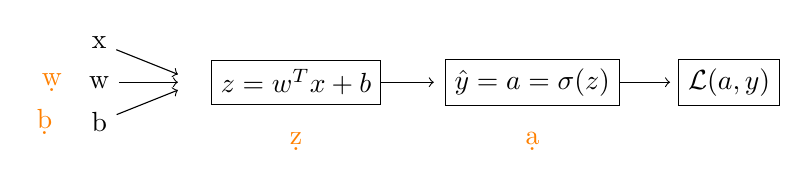
\begin{tikzpicture}
  \node (x) at (0, 1) {x};
  \node (w) at (0, .5) {w};
  \node (b) at (0,0) {b};
  \node [left = .1cm of w] {\color{orange}$\d w$}; 
  \node [left = .25cm of b] {\color{orange}$\d b$}; 
  \draw[->] (x) to (1, .6);
  \draw[->] (w) to (1, .5);
  \draw[->] (b) to (1, .4);
  \node[draw=black,rectangle] (z) at (2.5, .5) {$z = w^Tx + b$};
  \node at (2.5,-0.25) {\color{orange}$\d z$};
  \draw[->] (z) to (4.25, .5);
  \node[draw=black,rectangle] (yhat) at (5.5, .5) {$\hat y = a = \sigma(z)$};
  \node at (5.5,-0.25) {\color{orange}$\d a$};
  \draw[->] (yhat) to (7.25, .5);
  \node[draw=black,rectangle] (loss) at (8, .5) {$\mathcal L (a,y)$};
\end{tikzpicture}   \end{figure}
\newline
Note that $\d z = \d a \cdot g'(z)$ where $g(z) = \sigma(z)$, i.e. we use the fact that $\frac{\d L(a,y)}{\d z} = \frac{\d L(a,y)}{\d a} \frac{\d a}{\d z}$.

\paragraph{Two Layer Neural Network Back Propagation}
Let us now reconsider our two layer neural network and 
its computation graph. We highlight terms we must compute in \color{orange}{orange}\color{black}.
\begin{figure}[h]
\hspace{-20pt}
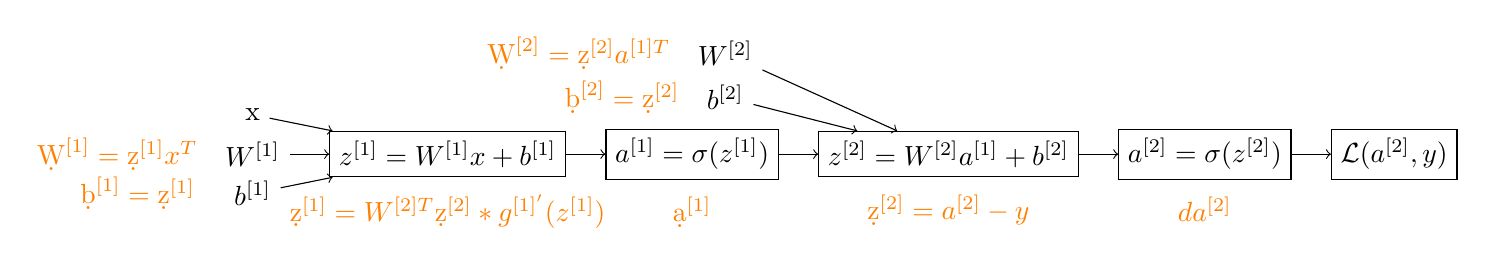
\begin{tikzpicture}
  \node (x)  at (-3, 1)  {x};
  \node (w1) at (-3, .5) {$W^{[1]}$};
  \node (b1) at (-3,0)   {$b^{[1]}$};
  \node [left = .1cm of w1] {\color{orange}$\d W^{[1]}= \d z^{[1]} x^T$}; 
  \node [left = .25cm of b1] {\color{orange}$\d b^{[1]}= \d z^{[1]}$}; 
  \node[draw=black,rectangle, right = .5cm of w1] (z1)  {$z^{[1]} = W^{[1]}x + b^{[1]}$};
  \draw[->] (x) to (z1);
  \draw[->] (w1) to (z1);
  \draw[->] (b1) to (z1);
  \node [below = .1cm of z1] {\color{orange}$\d z^{[1]}=W^{[2]T} \d z^{[2]} * g^{[1]'}(z^{[1]})$};
  \node[draw=black,rectangle, right = .5cm of z1] (a1) {$a^{[1]} = \sigma(z^{[1]})$};
  \draw[->] (z1) to (a1);
  \node [below = .1cm of a1] {\color{orange}$\d a^{[1]}$};
  \node[draw=black,rectangle, right = .5cm of a1] (z2) {$z^{[2]} = W^{[2]} a^{[1]} + b^{[2]}$};
  \node[below=.1cm of z2] (dz2) {\color{orange} $\d z^{[2]}= a^{[2]} - y$};
  \draw[->] (a1) to (z2);
  \node[above left = 1cm of z2] (w2) {$W^{[2]}$};
  \node[left = .1cm of w2] (dw2) {\color{orange}$\d W^{[2]}= \d z^{[2]} a^{[1]T}$};
  \node[below = .00025cm of w2] (b2) {$b^{[2]}$};
  \node[left = .1cm of b2] (db2) {\color{orange}$\d b^{[2]} = \d z^{[2]}$};
  \draw[->] (w2) to (z2);
  \draw[->] (b2) to (z2);
  \node[draw=black,rectangle,right = .5cm of z2] (a2) {$a^{[2]} = \sigma(z^{[2]})$};
  \node[below=.1cm of a2] (da2) {\color{orange} $da^{[2]}$};
  \draw[->] (z2) to (a2);
  \node[draw=black,rectangle,right=.5cm of a2] (loss) {$\mathcal{L}(a^{[2]}, y)$};
  \draw[->] (a2) to (loss);
\end{tikzpicture}   
\end{figure}
\newline
Where in $\d z^{[1]}=W^{[2]T} \d z^{[2]} * g^{[1]'}(z^{[1]})$ the $*$ denotes an element-wise product.
Note that the computations for $\d a^{[\ell]}$ are typically rolled into the next computation for $\d z^{[\ell]}$.
Further realize that the above computations are performed for \emph{each} training example in our data set 
during gradient descent.
\paragraph{Vectorized Implementation}
We can vectorize our computations as follows.
\begin{align*}   \d Z^{[2]} &= A^{[2]} - Y \\
  \d W^{[2]} &= \frac{1}{m} \d Z^{[2]} {A^{[1]}}^T \\
  \d b^{[2]} &= \frac{1}{m} \texttt{np.sum}(\d Z^{[2]}\texttt{, axis = 1, keepdims = True}) \\
  \d Z^{[1]} &= {W^{[2]}}^T \d Z^{[2]} * g^{[1]'}(Z^{[1]}) \hspace{35pt} (* \textrm{ denotes an element-wise product})\\
  \d W^{[1]} &= \frac{1}{m} \d Z^{[1]} X^T \\ 
  \d b^{[1]} &= \frac{1}{m} \texttt{np.sum}(\d Z^{[1]}\texttt{, axis = 1, keepdims = True}) \end{align*}

\subsubsection{Random Initialization}
\paragraph{Why Initializing With Zeros Won't Work for $W$'s: Symmetric Neurons}
Note that initializing our weights matrix with zeros will prevent gradient descent from working. What happens? For any example, $a_1^{[1]} = a_2^{[2]}$, whence $\d z_1^{[1]} = \d z_2^{[2]}$. I.e. the hidden units are symmetrical, and $\d W = \begin{bmatrix}   u & v \\ u & v \end{bmatrix}$ and our weights matrix will have first row equal to the second row. By induction, no matter how many times we train our network, the neurons in the hidden layer will remain symmetric and no learning will take place. 
It turns out $b$ does not have this symmetry-breaking problem, and so we can initialize $b$'s to zeros.

\paragraph{Random Initialization}
Instead, if we initialize weights randomly, each neuron in each hidden layer will compute different functions. I.e. $W^{[1]} = $\texttt{np.random.randn((.,.)) * 0.01} where we apply an ad-hoc scaling factor. We prefer initializing weights to small values. Why? Suppose we are using either sigmoid or $\tanh$ activation functions then if $W$ initialized large, $Wx + b$ also large, whence $g(z)$ large and we yield saturated (near-zero) gradients; this means gradient descent and learning will be very slow. If we don't have any sigmoid or $\tanh$ activation functions, this is less of an issue. 

\section{Deep Learning: $L$-layer Neural Networks}

Let's consider a four layer neural network, depicted below in figure \ref{fig: fourlayernet}.
Let us define some notation. Let $L=4$ denote the number of layers in the network. The notation $n^{[\ell]} = \# \textrm{units in layer } \ell$.

\begin{figure}[h]   \centering
  \label{fig: fourlayernet}
  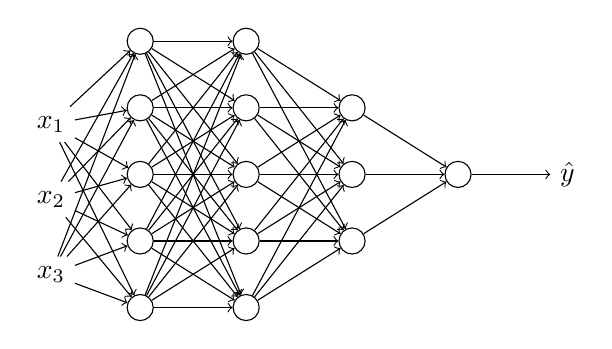
\begin{tikzpicture}[scale=0.25]     \node (x1) at (-2, 1) {$x_1$};
    \node [below = .5 cm of x1] (x2) {$x_2$};
    \node [below = .5 cm of x2] (x3) {$x_3$};
    \node [draw,circle,above right = 1 cm of x1] (n11) {};
    \node [draw,circle,below = .5 cm of n11] (n12) {};
    \node [draw,circle,below = .5cm of n12] (n13) {};
    \node [draw,circle,below = .5cm of n13] (n14) {};
    \node [draw,circle,below = .5cm of n14] (n15) {};
    \node [draw,circle,right = 1 cm of n11] (n21) {};
    \node [draw,circle,below = .5 cm of n21] (n22) {};
    \node [draw,circle,below = .5cm of n22] (n23) {};
    \node [draw,circle,below = .5cm of n23] (n24) {};
    \node [draw,circle,below = .5cm of n24] (n25) {};
    \node [draw,circle,right = 1cm of n22] (n31) {};
    \node [draw,circle,below = .5cm of n31] (n32) {};
    \node [draw,circle,below = .5cm of n32] (n33) {};
    \node [draw,circle,right = 1cm of n32] (outputneuron) {};
    \node [right = 1cm of outputneuron] (yhat) {$\hat y$};
    \draw[->] (x1) to (n11);
    \draw[->] (x1) to (n12);
    \draw[->] (x1) to (n13);
    \draw[->] (x1) to (n14);
    \draw[->] (x1) to (n15);
    \draw[->] (x2) to (n11);
    \draw[->] (x2) to (n12);
    \draw[->] (x2) to (n13);
    \draw[->] (x2) to (n14);
    \draw[->] (x2) to (n15);
    \draw[->] (x3) to (n11);
    \draw[->] (x3) to (n12);
    \draw[->] (x3) to (n13);
    \draw[->] (x3) to (n14);
    \draw[->] (x3) to (n15);
    \draw[->] (n11) to (n21);
    \draw[->] (n11) to (n22);
    \draw[->] (n11) to (n23);
    \draw[->] (n11) to (n24);
    \draw[->] (n11) to (n25);
    \draw[->] (n12) to (n21);
    \draw[->] (n12) to (n22);
    \draw[->] (n12) to (n23);
    \draw[->] (n12) to (n24);
    \draw[->] (n12) to (n25);
    \draw[->] (n13) to (n21);
    \draw[->] (n13) to (n22);
    \draw[->] (n13) to (n23);
    \draw[->] (n13) to (n24);
    \draw[->] (n13) to (n25);
    \draw[->] (n14) to (n21);
    \draw[->] (n14) to (n22);
    \draw[->] (n14) to (n23);
    \draw[->] (n14) to (n24);
    \draw[->] (n14) to (n25);
    \draw[->] (n15) to (n21);
    \draw[->] (n15) to (n22);
    \draw[->] (n15) to (n23);
    \draw[->] (n15) to (n24);
    \draw[->] (n15) to (n25);
    \draw[->] (n21) to (n31);
    \draw[->] (n21) to (n32);
    \draw[->] (n21) to (n33);
    \draw[->] (n22) to (n31);
    \draw[->] (n22) to (n32);
    \draw[->] (n22) to (n33);
    \draw[->] (n23) to (n31);
    \draw[->] (n23) to (n32);
    \draw[->] (n23) to (n33);
    \draw[->] (n24) to (n31);
    \draw[->] (n24) to (n32);
    \draw[->] (n24) to (n33);
    \draw[->] (n25) to (n31);
    \draw[->] (n25) to (n32);
    \draw[->] (n25) to (n33);
    \draw[->] (n31) to (outputneuron);
    \draw[->] (n32) to (outputneuron);
    \draw[->] (n33) to (outputneuron);
    \draw[->] (outputneuron) to (yhat);
  \end{tikzpicture}
  \caption{Four-layer, fully connected neural network.} \end{figure}
In our example depicted, $n^{[0]} = n_x = 3$, $n^{[1]} = n^{[2]} = 5$ and $n^{[3]} = 3$ and $n^{L} = 1$. We'll also use $a^{[\ell]} = g^{[\ell]}(z^{[\ell]})$ to denote the activations in layer $\ell$, where to compute $z^{[\ell]}$ we use weights matrix $W^{[\ell]}$ and bias term $b^{[\ell]}$. Lastly, realize that with this notation our input matrix $X = a^{[0]}$ and our output $\hat y = a^{[L]}$.

\paragraph{Forward Propagation}
In general, we have that for a single training example:
\begin{align*}   z^{[\ell]} &= W^{[\ell]} a^{[\ell-1]} + b^{[\ell]}, \\ 
  a^{[\ell]} &= g^{[\ell]}(z^{[\ell]}). \end{align*}
And for our entire training set, where $X = A^{[0]}$ is our data arranged such that each column is an observation:
\begin{align*}   Z^{[\ell]} &= W^{[\ell]} A^{[\ell-1]} + b^{[\ell]}, \\ 
  A^{[\ell]} &= g^{[\ell]}(Z^{[\ell]}).    \end{align*}
Note that by rules of matrix multiplication, it's easy to see that $Z^{[\ell]}$ must have as many columns as there are training examples, and since $g^{[\ell]}$ is applied element-wise then $A^{[\ell]}$ also has as $m$ columns.
For our last layer, $\hat Y = g(Z^{[L]}) = A^{[L]}$. We remark that although we typically try to vectorize code and remove \texttt{for}-loops, it is perfectly reasonable to loop over the layers in the network during forward propagation. I.e. we expect to see \texttt{for} $\ell = 1, \ldots, L$.

\paragraph{Getting Your Dimensions Right} In general, the dimension for a weights matrix at layer $\ell$ is given b
\begin{equation}   W^{[\ell]} : \left( n^{[\ell]}, n^{[\ell - 1]} \right). \end{equation}
What about our bias term? In general, $b^{[\ell]} : \left(n^{[\ell]}, 1\right)$, Further, during backpropogation, the dimensions of the derivative matrices don't change. I.e. 
$\d   W^{[\ell]} : \left( n^{[\ell]}, n^{[\ell - 1]} \right)$, and $\d b^{[\ell]} : \left(n^{[\ell]}, 1\right)$.

\paragraph{Deep Representations:
\small What do our intermediary layers come to learn in different applications?}
\begin{itemize} \item Consider face detection. The first layer of the network may learn to detect edges, and the second layer perhaps may learn how to detect different pieces of a face by connecting edges together such as an eye or an ear. A later layer of a network may learn to distinguish between faces at an even less granular level.

\item As another example consider problems in the context of audio. The first layer of the network may lrn to distinguish between low and high frequency waveforms, whereas the second layer may learn to recognize phonemes (in the word cat, each letter, when pronounced, is a phoneme), and later layers of the network may learn to recognize words and finally phrases/sentences.
\end{itemize}
Earlier layers are in general based on more granular features, i.e. simple transformations of the input data. Later layers compose hierarchically and are eventually able to solve complex tasks.   
\paragraph{Circuit Theory and Deep Learning}
``There are functions you can compute with a `small' $L$-layer deep neural network that shallower networks require exponentially more hidden units to compute.''

As an example, consider using a neural network to approximate \texttt{xor} applied to $n$ input bits. I.e. we seek to calculate $x_1 \textrm{ xor } x_2 \textrm{ xor } \ldots \textrm{ xor } x_n$. If we are free to use as many layers in the network as we wish, then we could envision building a \texttt{xor} tree as follows: pair successive inputs together and apply the \texttt{xor} operation, and pipe the resulting output into the subsequent layer of the network. Realize that we require $\log n$ layers in our network in order to exactly compute the right answer. If, on the other hand, we weren't allowed to use an arbitrary number of layers but instead only a single hidden layer, we would require $O(2^n)$ neurons in order to achieve the same result; to see why realize that we effectively need to enumerate all possible $2^n$ possible input sequences in order to map them correctly back to the right answer in a subsequent step. Note that it is possible to get away with using only $2^{n-1}$ neurons to accomplish this task but this is still exponentially more neurons than the network with $O(\log n)$ layers.

\paragraph{Hyperparameters}
The \emph{parameters} of a neural network are the weights and biases:
\[
W^{[1]}, b^{[1]}, W^{[2]}, b^{[2]}, \ldots, W^{[L]}, b^{[L]}. 
\]
But there are other factors which determine how these parameters are learned, and these in turn are called \emph{hyperparameters}. These include:
\begin{itemize} \item The learning rate $\alpha$.
\item The number of iterations of gradient descent that we run.
\item The number of hidden layers $L$.
\item The number of hidden units $n^{[1]}, n^{[2]}, \ldots, n^{[L]}$.
\item The choice of activation functions $g^{[1]}, g^{[2]}, \ldots, g^{[L]}$. \end{itemize}

In more advanced deep learning, additional hyperparameters include momentum, minibatch-size, and various forms of regularizations.
Applied deep learning is a very empirical process, which means that there is a loop: (i) idea, (ii) code, (iii) experiment; we iterate on this to find the best set of hyperparameters. It's nearly impossible to get these right on the first try, and so it's important that we set up a train, development, and test data set accordingly. The optimal configuration is often application/domain dependent.

\section{Setting up your Machine Learning Application}
\subsection{Splitting Data, and the (missing) Bias and Variance tradeoff}
\paragraph{Train, Development, and Test Data}
Historically, it was considered best practice to split data into training and test sets of size 70\% and 30\% respectively. This maybe makes sense when we have (up to) a million records. But with bigger data sets, we don't necessarily also need larger test sets in order to validate our algorithm; it may suffice to sample 10k records and use them as hold-out or test sets. If we believe in this example that 10k records is enough to deliver an unbiased estimate of which \emph{algorithm} is better (on the development/CV/hold-out set) and what the test error is (on the test set), then our split becomes more like 98\%, 1\%, 1\%. Lastly, we remark that it may be OK to not have a test set so long as we don't need an unbiased estimator of performance.
\vspace{-.5ex}
\paragraph{Bias - Variance} In Deep Learning, we still talk about bias and variance, but we don't emphasize as much that there is a tradeoff between these two quantities. Andrew considers \emph{bias} to be determined by the training set error relative to how well a human can perform the same task (i.e. Bayes error), and the \emph{variance} to be determined by the relation to the training set error. 
E.g. if \{\texttt{train, test}\} error is \{0.01, 0.11\} on a problem where humans can achieve perfect accuracy, we might say the algorithm has low bias but high variance. If we observe \{0.15, 0.16\}, we might say the algorithm has high bias. If we observe \{0.15, 0.30\}, we have a case of both high bias and high variance. Lastly, \{0.005, 0.01\} corresponds to both low bias and low variance.

\paragraph{Basic Recipe for Machine Learning}
Supposing that we have:
\begin{itemize}   \item \emph{High Bias}, as measured by the \emph{training} set. Possible remedies $\leadsto$ bigger network, more hidden units, train longer, and neural network architecture search.
  \item \emph{High Variance}, as measured by the \emph{development} set. Possible remedies $\leadsto$ more data, regularization, and neural network architecture search. \end{itemize}
Notice that depending on whether we have high bias or high variance, the set of things to try is very different. In modern deep learning, so long as we can train a bigger network on a bigger dataset this guarantees a model with lower bias \emph{and} lower variance, i.e. there is no longer a bias-variance tradeoff.

\subsection{Regularization} 
Suppose you have high variance. One way to address this is through regularization (another is through obtaining more training data, this may be harder but also more reliable). 
\paragraph{Logistic Loss with Regularization}
In this context, an $\ell_2$ regularization may look as follows:
\[
  J(w,b) = \frac{1}{m} \sum_{i=1}^m \mathcal L \left(\hat {y^{(i)}}, y^{(i)}\right) + \frac{\lambda}{2m} \|w\|_2^2
\]
where $\|w\|_2^2 = \sum_{j=1}^{n_x} w_j^2 = w^Tw$. Why not add regularization to $b$? Since $b \in \mathbb R$ just a single scalar, adding it to $w \in \mathbb R^{n_x}$ won't make much of a difference in practice ($w$ contains many real numbers whose magnitude overwhelm $b$). An $\ell_1$ regularization would look like $\frac{\lambda}{m} \sum_{i=1}^{n_x} |w_i|$. With $\ell_1$ regularization, we yield a \emph{sparse} model.
In all the above, $\lambda$ is the regularization hyper-parameter which is set using the cross-validation set.

\paragraph{Neural Network Regularization} Here,
\[
J\left(W^{[1]}, b^{[1]}, \ldots, W^{[L]}, b^{[L]}\right) = \frac{1}{m} \sum_{i=1}^{m} \mathcal L(\hat {y^{(i)}}, y^{(i)}) + \frac{\lambda}{2m} \sum_{\ell=1}^{L} \|W^{[\ell]}\|_F^2
\]
where we're using Frobenius norm $\|W^{[\ell]}\|_F^2 = \sum_{i=1}^{n^{[\ell-1]}} \sum_{j=1}^{n^{[\ell]}} (W_{ij}^{[\ell]})^2$, recalling that $W \in \mathbb R^{n^{[\ell]} \times n^{[\ell - 1]}}$. We need to make note that we have a new rule for back-propagation:
\[
\d W^{[\ell]} = \left(\texttt{from backprop}\right) + \frac{\lambda}{m} W^{[\ell]}.
\]
We sometimes refer to adding this regularization term as \emph{weight decay}, since the back propagation update rule becomes
\[
W^{[\ell]} := W^{[\ell]} - \alpha \d W^{[\ell]} = \underbrace{W^{[\ell]} - \frac{\alpha \lambda}{m} W^{[\ell]}}_{(1-\frac{\alpha \lambda}{m})W^{[\ell]}} - \alpha \left(\textrm{from backprop}\right)
\]
where $(1-\frac{\alpha \lambda}{m}) < 1$ is a shrinkage term.

\paragraph{Why does Regularization Mitigate Overfitting?} As we crank up $\lambda$, we push $W \leadsto 0$, whence the effects of hidden units are mitigated, and we realize a network that behaves closer to a stacked (multiple layers) logistic regression. 
Another way to gain intuition is as follows. Suppose we use a $\tanh$ activation function. If $\lambda \uparrow$, then $W^{[\ell]} \downarrow$, whence our input values to $\tanh$ are very small. Recall that $\tanh$ is approximately linear around the origin, and so for high levels of $\lambda$ we recover a neural network where every layer is linear; recall that no matter how deep the network is if it only consists of linear layers then the whole network yields a linear decision boundary.

\paragraph{(Inverted) Dropout Regularization} For \emph{each} training example, and for \emph{each} neuron in our network, we toss a (weighted) coin and remove the neuron from the network entirely according to the 
outcome. This means that for each training example we perform back propagation on a modified and (sometimes significantly) 
reduced network.
One way to implement dropout is known as ``inverted dropout''. We illustrate with layer $\ell = 3$, for some \texttt{keep\_prob} 
e.g. 0.8.

\begin{verbatim} 
d3 = np.random.rand(a3.shape[0], a3.shape[1]) < keep_prob  # rand, NOT randn.
a3 = np.multiply(a3, d3)
a3 /= keep_prob  # <-- Inverted dropout technique.
\end{verbatim}
The last step is what gives the technique its name, and is 
simply done in order to keep, in expectation, $z^{[4]} = W^{[4]} a^{[3]} + b^{[b]}$ the same. Note that this Boolean array \texttt{d3} is also used in back-propagation. 
Now, if we are to make predictions given a new $X = a^{[0]}$, \emph{we don't need to   apply drop-out at test time.}

\paragraph{Why does dropout work?} One intuition is that in applying dropout, we prevent our network from relying on any one particular feature too much and instead spread out the weights. We can think about this from the perspective of a single neuron in a network: since the neurons in the previous layer can be randomly eliminated, the neuron in the subsequent layer must learn not to place too much weight on any one feature and instead learn a small amount of information from each. This spread of weights has the effect of shrinking the squared norm of the weights matrix; in fact, dropout can be formally shown tobe an adaptive form of $\ell_2$ regularization.

\paragraph{Varying dropout by layer}
Note that it's also possible to vary the \texttt{keep\_prob} variable by layer. In fully connected layers with more neurons where we might worry about overfitting more, it's sensible to apply a more stringent (lower) value of \texttt{keep\_prob} when compared to perhaps a succession of layers with decreasingly fewer neurons where perhaps we are worried about overfitting less. The downside of this approach is that we have additional hyperparameters to search through when cross validating our approach; a workaround is to make a binary decision of whether to apply dropout at all to a given layer, and for all layers with dropout applied to use the same \texttt{keep\_prob}. We lastly remark that dropout \emph{can} be applied to the input features, but typically if any is applied we choose \texttt{keep\_prob} $\approx 1$.
One downside to dropout is that our cost function $J$ is no longer well defined, and we are not guaranteed that $J$ will be monotone decreasing as a function of the number of iterations of gradient descent.

\paragraph{Backpropagation with Dropout} There are two steps to carry out for each layer which utilizes dropout.
\begin{itemize} \item We previously shut down some neurons during forward propagation with mask $D^{[\ell]}$; in back propagation, we have to shut down the same neurons by applying the same mask $D^{[\ell]}$ to $\d A^{[\ell]}$.
\item During forward propagation we had previously divided $A^{[\ell]}$ by \texttt{keep\_prob}, whence in backward propagation we must divide $\d A^{[\ell]}$ by \texttt{keep\_prob} again (since $\frac{\d\,}{\d x} c f(x) = c \frac{\d\,}{\d x} f(x)$). \end{itemize}

\subsection{Other Regularization Methods} 
\paragraph{Data augmentation} E.g. in computer vision we can flip, rotate, and zoom into images to increase the size of our training set. By applying random distortions, we can fake additional training example. Of course, an independent training example provides more information than a synthesized example. In recognizing hand-written text, we could also apply small rotations and random perturbations to the ``thickness'' of the lines drawn. 

\paragraph{Early Stopping}
Another technique of regularization is \emph{early stopping}, whereby optimize for training error loss but also evaluate our cross-validation dataset error each iteration, and stop training when development set error starts increasing. Why does this method work? In practice, we initialize $W$ to small random numbers, and as we train more iterations of gradient descent we learn larger weights; by stopping early, we are in turn applying a shrinkage effect and encouraging a smaller Frobenius norm on $W$. Andrew likes to keep the task of Optimizing Cost Function $J(W,b)$ separate from the task of Not Overfitting, since each has its own set of workarounds; see orthogonalization.

\section{Setting Up Your Optimization Problem}
\subsection{Normalizing input data}
Suppose we have a two dimensional data-set as follows; we plot out $(x_1, x_2)$ pairs.

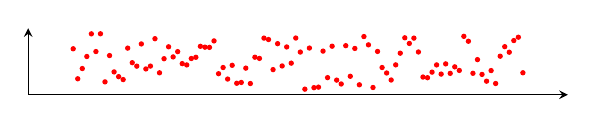
\begin{tikzpicture}[     declare function={a(\x)=0.75;},     declare function={b(\x)=0.25;} ] \begin{axis}[     domain=1:5,     axis lines=middle,     axis equal image,     xtick=\empty, ytick=\empty,     enlargelimits=true,     clip mode=individual, clip=false ] \addplot [red, only marks, mark=*, samples=100, mark size=0.75]     {0.5*(a(x)+b(x)) + 0.5*rand*(a(x)-b(x))}; \end{axis} \end{tikzpicture}

We standardize our data by first subtracting out the mean: $\mu = \frac{1}{m} \sum_{i=1}^{m} x^{(i)}$, $x -= \mu$.

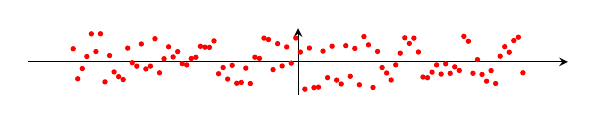
\begin{tikzpicture}[     declare function={a(\x)=0.25;},     declare function={b(\x)=-0.25;} ] \begin{axis}[     domain=-2:2,     axis lines=middle,     axis equal image,     xtick=\empty, ytick=\empty,     enlargelimits=true,     clip mode=individual, clip=false ] \addplot [red, only marks, mark=*, samples=100, mark size=0.75]     {0.5*(a(x)+b(x)) + 0.5*rand*(a(x)-b(x))}; \end{axis} \end{tikzpicture}

We then divide through by the variance, $\sigma^2 = \frac{1}{m} \sum_{i=1}^{m} x^{(i)}**2$ where we remark that the $**$ denotes element-wise multiplication and further that typically $\textrm{Var}(Z) = \mathbb E [Z^2] - \mathbb E [Z]^2$, but we've already de-meaned our random vector.
$x /= \sigma^2$.
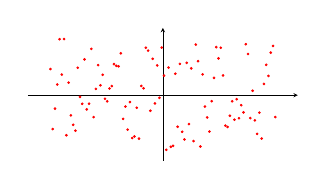
\begin{tikzpicture}[scale=0.5,     declare function={a(\x)=0.25;},     declare function={b(\x)=-0.25;} ] \begin{axis}[     domain=-.5:.5,     axis lines=middle,     axis equal image,     xtick=\empty, ytick=\empty,     enlargelimits=true,     clip mode=individual, clip=false ] \addplot [red, only marks, mark=*, samples=100, mark size=0.75]     {0.5*(a(x)+b(x)) + 0.5*rand*(a(x)-b(x))}; \end{axis} \end{tikzpicture}

We remark that the same $\mu$ and $\sigma^2$ should be used to normalize the development and test data-sets.

\paragraph{Normalization and Gradient Descent} Why should we normalize our data? It comes down to being able to apply a higher learning rate when training our algorithm. When our input data $x_1, x_2$ have very different scales (e.g. $x_1 \in [0, 1e3]$ and $x_2 \in [0,1]$), the weights learned for $w_1$ and $w_2$ will be on very different scales as well. If we plot the loss function $\mathcal L(\hat y, y)$ over $w_1, w_2$ it turns out that we end up with very elongated contours. We therefore must apply a small learning rate, leading to many small steps before convergence.

\begin{minipage}{1.0\textwidth} \begin{multicols}{2} 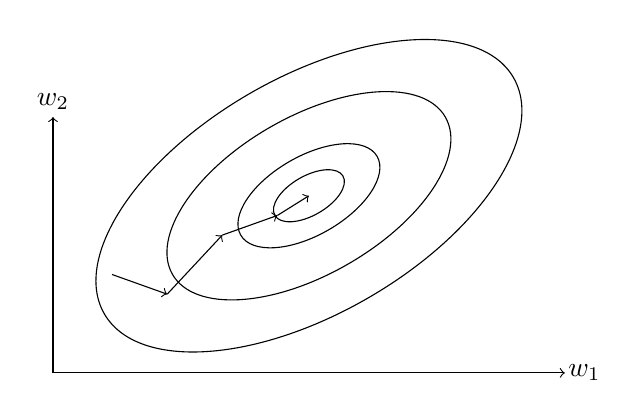
\begin{tikzpicture}
  \draw[->] (-3.25,-2.25) to (-3.25, 1);
  \node at (-3.25, 1.2) {$w_2$};
  \draw[->] (-3.25,-2.25) to (3.25, -2.25);
  \node at (3.5, -2.25) {$w_1$};
    \draw[rotate=30] (0,0) ellipse (3cm and 1.5cm); 
    \draw[rotate=30] (0,0) ellipse (2cm and 1cm);     \draw[rotate=30] (0,0) ellipse (1cm and .5cm); 
    \draw[rotate=30] (0,0) ellipse (.5cm and .25cm);
  \draw[->] (-2.5, -1) to (-1.8, -1.25);
  \draw[->] (-1.8, -1.25) to (-1.1, -.5);
  \draw[->] (-1.1, -.5) to (-.4, -.25);
  \draw[->] (-.4, -.25) to (0, 0);
\end{tikzpicture} 
\vfill\null \columnbreak
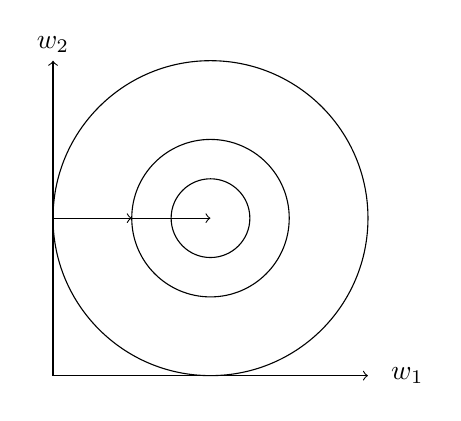
\begin{tikzpicture}[scale=2]
  \draw[->] (-1, -1) to (-1, 1);
  \node at (-1, 1.1) {$w_2$};
  \draw[->] (-1, -1) to (1, -1);
  \node at (1.25, -1) {$w_1$};
  \draw (0, 0) circle (1cm);   
  \draw (0, 0) circle (.5cm); 
  \draw (0, 0) circle (.25cm); 
  \draw[->] (-1, 0) to (-.5, 0);
  \draw[->] (-.5, 0) to (0, 0);
\end{tikzpicture}
\end{multicols} \end{minipage}

Whereas if we first normalize our inputs, the loss function when plotted over the weights appears more like a uniform bowl, and our contour plots are spherical. Our learning rate can be set higher since the step size is no longer limited by the major axis. Performing normalization never hurts our learning algorithm.

\subsection{Vanishing/Exploding gradients}
Suppose for the sake of argument that we have a very deep neural network; we've drawn only two hidden neurons per layer but this is only for illustration sake.

{
\centering
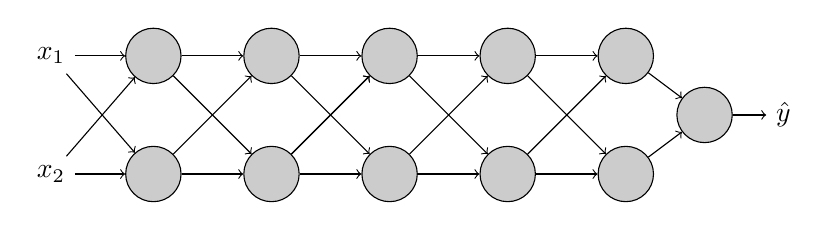
\begin{tikzpicture}[darkstyle/.style={circle,draw,fill=gray!40,minimum size=20}]
  \node (x1) at (-1.3, 1.5) {$x_1$};   \node (x2) at (-1.3, 0) {$x_2$};   
  \foreach \x in {0,...,4}     \foreach \y in {0,...,1}
      \node [darkstyle] (\x\y) at (1.5*\x,1.5*\y) {};
  \draw[->] (x1) to (00);
  \draw[->] (x1) to (01);
  \draw[->] (x2) to (00);
  \draw[->] (x2) to (01);
  \draw[->] (00) to (10);
  \draw[->] (00) to (11);
  \draw[->] (01) to (10);
  \draw[->] (01) to (11);
  \draw[->] (10) to (21);
  \draw[->] (10) to (20);
  \draw[->] (10) to (21);
  \draw[->] (11) to (20);
  \draw[->] (11) to (21);
  \draw[->] (20) to (30);
  \draw[->] (20) to (31);
  \draw[->] (21) to (30);
  \draw[->] (21) to (31);
  \draw[->] (30) to (40);
  \draw[->] (30) to (41);
  \draw[->] (31) to (40);
  \draw[->] (31) to (41);
  \node[darkstyle] (outputneuron) at (7, .75) {}; 
  \draw[->] (40) to (outputneuron);
  \draw[->] (41) to (outputneuron);
  \node (yhat) at (8, .75) {$\hat y$};
  \draw[->] (outputneuron) to (yhat);
\end{tikzpicture}
}

Suppose we choose $g(z) = z$, i.e. a linear activation function, and suppose for sake of argument that we ignore our bias term, i.e. $b^{[\ell]} = 0$ for each layer. It's easy to see that $\hat y = W^{[L]} W^{[L-1]} \ldots W^{[2]} W^{[1]} W^{[0]} X$. Ignoring the last $W^{[L]}$ which is of different dimension, suppose each intermediary weight matrix is slightly larger than an identity matrix i.e. $\begin{bmatrix}   1 + \epsilon & 0 \\ 0 & 1 + \epsilon \end{bmatrix}$ then the value of $\hat y$ explodes with the number of layers,
$\hat y = W^{[L]} \begin{bmatrix}   (1 + \epsilon)^{L-1} & 0 \\ 0 & (1 + \epsilon)^{L-1} \end{bmatrix}X$. Similarly, if the intermediary matrices are slightly smaller than an identity matrix, then the values of subsequent activation functions get exponentially smaller. This can start to become problematic if we have $L$ quite large; in 2018 Microsoft published state of the art results using $L \approx 150$, which is large enough for these problems to manifest by slowing down gradient descent.

\subsection{Weight Initialization for Deep Networks} Suppose for the sake of illustration we have a single activation neuron.
\begin{figure}[h]
  \centering   
  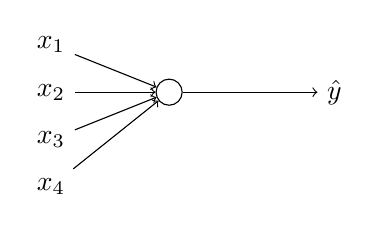
\begin{tikzpicture}[scale=0.6]
    \node (x1) at (-1, 1) {$x_1$};
    \node (x2) at (-1, 0) {$x_2$};
    \node (x3) at (-1,-1) {$x_3$};
    \node (x4) at (-1,-2) {$x_4$};
    \node[draw,circle] (neuron) at (1.5,0) {};
    \draw[->] (x1) to (neuron);
    \draw[->] (x2) to (neuron);
    \draw[->] (x3) to (neuron);
    \draw[->] (x4) to (neuron);
    \node (output) at (5,0) {$\hat y$};
    \draw[->] (neuron) to (output);
  \end{tikzpicture} 
\end{figure}
For simplicity sake, ignore $b$ for now. The input to our activation function
looks like $z = w_1 x_1 + w_2 x_2 + \ldots + w_n x_n$. So, if the number of input features (or hidden neurons in an intermediary layer) is large, we want smaller $w_i$ to compensate such that $z$ doesn't explode. One idea might be to set $\textrm{Var}(w_i) = \frac{1}{n}$ such that $\textrm{Var}(z) \approx \sum_i \textrm{Var}(x_i)$ and we preserve the variance of our input to our activation function. To accomplish this, we set
\begin{align*}   W^{[\ell]} = \texttt{np.random.randn(shape) * np.sqrt} \left(\frac{1}{n^{[\ell-1]}}\right) \end{align*}
If we're using ReLU activation functions, it's common to replace the numerator in the scaling constant above with a 2 instead of a 1 (i.e. to set $\textrm{Var}(w_i) = \frac{2}{n}$). If you want, you can consider this scaling factor to be another hyperparameter, and we can search across a sequence of values and choose the best according to our development data-set.

\subsection{Numerical Approximation of Gradients}
When performing back propagation, there is a technique known as Gradient-Checking
that will help to ensure your implementation of back propagation is correct. To 
perform gradient checking, we first need to understand how to numerically approximate
a gradient.

Suppose we have some function $f(\theta) = \theta^3$, and we choose $\epsilon = 0.01$. To compute a numerical gradient around a point $\theta$, we will use a central difference method:
\[
f'(\theta) \approx \frac{f(\theta + \epsilon) - f(\theta - \epsilon)}{2 \epsilon}.
\]
This approximation has an error that is upper-bounded by $O(\epsilon^2)$, which can be shown through a Taylor Series approximation (see \href{https://en.wikipedia.org/wiki/Finite_difference_method#Accuracy_and_order}{finite difference method}), recalling that $f'(\theta) = \lim_{\epsilon \to 0} \frac{f(\theta + \epsilon) - f(\theta - \epsilon)}{2 \epsilon}$. This is in stark contrast to taking a one-sided difference to approximate a gradient, which has error bounded by $O(\epsilon)$.

\paragraph{Gradient Checking} A technique for catching errors in a back-propagation implementation. The first step is to take
$W^{[1]}, b^{[1]}, \ldots, W^{[L]}, b^{[L]}$ and \emph{reshape} 
them into one giant vector, call it $\theta$. We may now 
equivalently define our cost function as 
 $J(W^{[1]}, b^{[1]}, \ldots, W^{[L]}, b^{[L]}) = J(\theta)$.
The next step is to take $\d W^{[1]}, \d b^{[1]}, \ldots, \d W^{[L]}, \d b^{[L]}$ (ordered the same way) and reshape them into another giant vector $\d \theta$.

\begin{algorithm}
  \caption{\texttt{Grad-check}}   \For{each $i$} {
    $\d \theta_{\texttt{approx}}^{[i]} = \frac{J(\theta_1, \theta_2, \ldots, \theta_i + \epsilon, \ldots) - J(\theta_1, \theta_2, \ldots, \theta_i - \epsilon, \ldots)}{2\epsilon}$
  } \end{algorithm}
We now end up with two vectors, each the same length, $\d \theta_{\texttt{approx}}^{[i]}$ and $\d \theta$. We can now compare them using Euclidean norms,
\begin{equation}
\label{eq: normed-diff}
\frac{\| \d \theta_{\texttt{approx}} - \d \theta\|_2}{\|\d \theta_{\texttt{approx}}\|_2 + \| \d \theta \|_2}
\end{equation}

Now, suppose we implement gradient checking with $\epsilon = 10^{-7}$. If \ref{eq: normed-diff} is $O(10^{-7})$ or smaller, then great! We've implemented back propagation correctly. If \ref{eq: normed-diff} outputs something $O(10^{-5})$, it would be prudent to check the components (elements) of $\d \theta_{\texttt{approx}} - \d \theta\|_2$ and see if any one of them is particularly large, if so we might want to double check our implementation for that layer. If, however, \ref{eq: normed-diff} outputs something $O(10^{-3})$, it's indicative of a bug in our implementation. Again, the method is to inspect the components of \ref{eq: normed-diff} to locate the source of our bug.

\paragraph{Implementation Notes for Gradient Checking}
\begin{itemize}   \item Don't use in training -- only to debug. I.e. computing $\d \theta_{\texttt{approx}}^{[i]}$ for each $i$ is expensive. Once we've verified that \ref{eq: normed-diff} outputs something sufficiently small, we should turn \emph{off} \texttt{grad-check}.
  \item If algorithm fails \texttt{grad-check}, examine individual components in order to debug. We might find that the bug is isolated to a particular layer. 
  \item Remember regularization -- if $J(\theta) = \frac{1}{m} \sum_{i=1}^m \mathcal L(\hat {y^{(i)}}, y^{(i)}) + \frac{\lambda}{2m} \sum_\ell \|W^{[\ell]}\|_F^2$ includes regularization, then we need to be sure to include this penalty term when we compute $\d \theta_{\texttt{approx}}$, since $\d \theta$ is defined as the derivative with respect to our cost function.
  \item \texttt{Grad-check} does \emph{not} work with dropout -- since dropout randomly eliminates (hidden) nodes from the network, there is no easy to compute $J(\theta)$ that dropout is doing gradient descent on.\footnote{It turns out that when using dropout, we can actually define a cost function that is defined over the exponentially large space of all possible subsets of hidden neurons, however this is computationally intractable to compute and compare with.} To get around this, we might turn \texttt{keep\_prop = 1.0} before running \texttt{grad-check}.
  \item Run at a random initialization of $W$'s and $b$'s, and perhaps again after some training -- it's possible that our (buggy) back propagation algorithm may not incur \emph{too} much error when $W, b \approx 0$, but that as our weights increase the errors do to. So, we might try running \texttt{grad-check} when we first randomly initialize $W$ and $b$, and then also again after some training has allowed our weights to drift sufficiently away from zero.  \end{itemize}

\section{Optimization Algorithms}
\subsection{Mini-batch gradient descent}
We've previously seen that matrix-multiplies allow us to efficiently compute a gradient on all $m$ training examples simultaneously. I.e., we had
\begin{equation}
  X = \begin{bmatrix}     x^{(1)} & x^{(2)} & \ldots & x^{(m)}   \end{bmatrix} \in \mathbb R^{n_x, m} \\ \hspace{15pt}
  Y = \begin{bmatrix}     y^{(1)} & y^{(2)} & \ldots & y^{(m)}   \end{bmatrix} \in \mathbb R^{1, m}.
\end{equation}

But in deep learning we often work with large data; 
what if $m$ really large, e.g. 50M? This means that we have to churn through a lot of compute before taking a very small step in gradient descent. It turns out that we can often allow our algorithm to learn faster if we allow for gradient descent to start taking palce before we're done processing all $m$ training examples.

We partition our data into mini-batches, 
each of approximately equal size. Let us use a superscript curly-brace to denote the mini-batch number. E.g. if we choose a mini-batch size of 1e3 training examples, 
our training data now looks like
\[
  X = \begin{bmatrix}       \color{purple} x^{(1)} & \color{purple} x^{(2)} & \color{purple} \ldots & \color{purple} x^{(1000)}      & \color{orange} x^{(1001)} & \color{orange} \ldots & \color{orange} x^{(2000)} & \color{black} \ldots & x^{(m)}   \end{bmatrix} \in \mathbb R^{n_x, m}
\]
and correspondingly for $Y$.
The number of mini-batches is of course given by $m/\texttt{mini-batch size}$. Mini-batch $t$ then consists of $\{X^{\{t\}}, Y^{\{t\}}\}$. The dimension of $X^{\{t\}}$ is $(n_x, \texttt{mini-batch size})$.

\begin{algorithm}[h]   \caption{Mini-batch gradient descent}
  \For{$t = 1, \ldots, m/\texttt{mini-batch size}$} {
    \tcp{One step (epoch) of gradient descent using $X^{\{t\}}, Y^{\{t\}}$.}
    $Z^{[1]} = W^{[1]} X^{\{t\}} + b^{[1]}$ \\
    $A^{[1]} = g^{[1]}(Z^{[1]})$ \\
    $\vdots$ \\
    $A^{[L]} = g^{[L]}(Z^{[L]})$
    $J^{\{t\}} \gets \frac{1}{\texttt{mini-batch size}} \sum_{i=1}^{\texttt{mini-batch size}} \mathcal L(\hat y^{(i)}, y^{(i)}) + \frac{\lambda}{2 \cdot \texttt{mini-batch size}} \sum_{\ell = 1}^{L} \|W^{[\ell]}\|_F^2$ \\
    \tcp{Backpropagation to compute gradients w.r.t. $J^{\{t\}}$ (using $X^{\{t\}}, Y^{\{t\}}$).}
    $W^{[\ell]} := W^{[\ell]} - \alpha \d W^{[\ell]}$
    $b^{[\ell]} := b^{[\ell]} - \alpha \d b^{[\ell]}$
  } \end{algorithm}

With larger data sets, mini-batch gradient descent is likely to converge much faster.

\subsubsection{Understanding mini-batch gradient descent}
With (vanilla) batch gradient descent, we expect that the loss
function should be monotone decreasing with respect to the 
number of iterations of gradient descent. E.g.
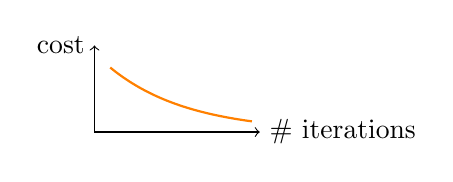
\begin{tikzpicture}
\draw[->] (0, 0) to (0, 1.1) node [left] {cost}; \draw[->] (0, 0) to (2.1, 0) node [right]{\# iterations}; 
\draw[smooth, domain=0.2:2, color=orange, thick]      plot (\x,{exp(-\x)}) {};
\end{tikzpicture}
When we train on a cost function $J^{\{t\}}$, it depends on
$X^{\{t\}}, Y^{\{t\}}$ which vary with each iteration. And so
it's not the case that we expect our cost function to 
monotonically decrease with each iteration of mini-batch gradient descent. We should see something that is (hopefully) sinusoidal and downward trending, e.g.
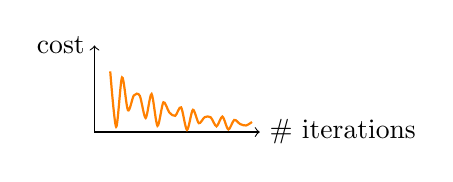
\begin{tikzpicture}
\draw[->] (0, 0) to (0, 1.1) node [left] {cost}; \draw[->] (0, 0) to (2.1, 0) node [right]{\# iterations};
\draw[smooth, domain=0.2:2, color=orange, thick]
plot (\x,{exp(-\x)*abs(cos(\x*1000))}) {};
\end{tikzpicture}. Why does our learning plot have this shape? It could be the case that the first epoch of data $X^{\{1\}}, Y^{\{1\}}$ was ``easier'' to predict on relative to a latter epoch.


\subsubsection{Choosing mini-batch size}
One point worth discussing is how to choose your mini-batch size. If we select $\texttt{mini-batch size} = m$, then we recover gradient descent. On the other extreme, we can set the \texttt{mini-batch size} to $1$, in which case we get 
\href{https://en.wikipedia.org/wiki/Stochastic_gradient_descent}{Stochastic Gradient Descent}, in which case each 
training example is its own mini-batch. Let's consider these two extremes as applied to the following hypothetical loss function (and corresponding contours).
{
\begin{figure}[h]
\centering
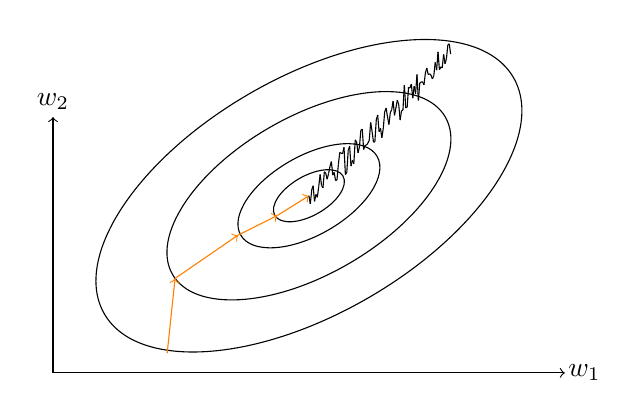
\begin{tikzpicture}
      \draw[->] (-3.25,-2.25) to (-3.25, 1);
      \node at (-3.25, 1.2) {$w_2$};
      \draw[->] (-3.25,-2.25) to (3.25, -2.25);
      \node at (3.5, -2.25) {$w_1$};
      \draw[rotate=30] (0,0) ellipse (3cm and 1.5cm); 
      \draw[rotate=30] (0,0) ellipse (2cm and 1cm);     \draw[rotate=30] (0,0) ellipse (1cm and .5cm); 
      \draw[rotate=30] (0,0) ellipse (.5cm and .25cm);
  \draw[->,orange] (-1.8, -2) to (-1.7, -1.05);
  \draw[->,orange] (-1.7, -1.05) to (-.9, -.5);
  \draw[->,orange] (-.9, -.5) to (-.4, -.25);
  \draw[->,orange] (-.4, -.25) to (0, 0);
  \NewDocumentCommand{\irregularline}{O {2mm} m m D <> {20}}{{       \coordinate (old) at #2;       \foreach \i in {1,2,...,#4}{         \draw (old) -- ($ ($#2!\i/(#4+1)!#3$) + (0,#1*rand) $) coordinate (old);       }       \draw (old) -- #3;     }}
  \irregularline{(0,0)}{(1.8,1.8)}<100>
\end{tikzpicture} 
\end{figure}
}

We've drawn vanilla gradient descent (in \color{orange}{orange}\color{black}) taking a few easy steps through the training data, each time moving toward the 
(global) minimum. On the other hand stochastic gradient descent (which we've drawn starting from a different initialization point for the sake of illustration) 
doesn't always get the direction right and in fact the path may be
far more circuitous than what we've shown. In fact, SGD won't even ever hit the global minimum (or ``converge''), it is far more likely to simply ``dance around'' the global minimum within some reasonably tight radius.

\paragraph{Advantages of mini-batch gradient descent}
In reality, we choose a mini-batch size in between 1 and $m$. If we were to choose $m$, the time required for each step of 
training would be too large (assuming large data). If we were to choose SGD, the downside is that we lose almost all speed-up from 
vectorization, since we process only one example at a time. With mini-batch gradient descent, we do get some 
vectorization (speed-up relative to processing one example at a time), and secondly we can make progress without 
waiting to process the entire training set. Further, with mini-batch gradient descent we won't take as circuitous a 
route before approaching the global optimum (which again we will not hit exactly).

\begin{itemize}   
  \item If training set is small (e.g. less 2,000 observations), just use batch gradient descent since the whole training set can be processed quite quickly.
  \item Otherwise, consider picking a mini-batch size equal to a power of two, such that hopefully data can 
    be loaded and stored in cache (or GPU memory), perhaps in the set $\{2^6, \ldots, 2^9\}$. 
\end{itemize}

\subsection{Momentum and Exponentially Weighted (moving) Averages} There are faster algorithms relative to mini-batch gradient descent.
To understand them, we need to understand \href{https://en.wikipedia.org/wiki/Moving_average#Exponential_moving_average}{exponentially weighted averages}. Suppose we have a time-series dataset  $x_1, \ldots, x_T$; we might estimate a moving average as follows:
\begin{align}
  \label{eq: expmovavg}   v_0 &= 0 \nonumber \\
  v_i &= 0.9 * v_{i-1} + 0.1 * x_i \hspace{35pt} \texttt{for } i > 0. \end{align}

We can make this a little bit more interesting by choosing some $\beta$ and then setting our update rule to become $v_i = \beta * v_{i-1} + (1-\beta) * x_i$. It can be shown that $v_t$ is an average over approximately $\frac{1}{1-\beta}$ points of data. As we set $\beta \approx 1$, we average over more points of data and get a \emph{smoother} time-series. The downside of averaging over more points is that we learn the trend of our data \emph{slower} (and therein incur a higher latency bias).

\paragraph{Math behind exponentially weighted averages} Let's unroll our formula to 
gain an intuition for what's happening. Suppose we have 100 data points.
\begin{align*}   v_{100} &= \beta v_{99} + (1-\beta) x_{100} \\
  v_{99}  &= \color{purple} \beta v_{98} + (1-\beta) x_{99} \\ 
  &\ldots \end{align*}
Then we can rewrite our last value as 
\[
  v_{100} = (1-\beta) x_{100} + \beta \left( \color{purple} (1-\beta) x_{99} + \beta v_{98} \color{black} \right) 
\]
and continuing to unroll term-by-term we see that
\[
  v_{100} = (1-\beta) x_{100} + (1-\beta) \beta x_{99} + (1-\beta) \beta^2 x_{98} + (1-\beta) \beta^3 x_{97} + \ldots.
\]

Put differently, the time series of data-points $v_i$ are generated by taking the element-wise product of our original time series with an exponentially decaying function which places the most weight on the most recent data point (and decaying weight to older data points). The coefficients add up to one, less a bias term that will be discussed later. In practice, to compute \ref{eq: expmovavg}- we only need to store a single real number in memory which we continuously update to take on the latest value of 
the moving average (based on its last value and the most recent data).

\paragraph{Bias correction in exponentially weighted (moving) averages} Let's consider our recurrence \ref{eq: expmovavg}. Notice that since we initialize $v_0 = 0$, and since $\beta \in (0,1)$, then
\begin{align*}   v_1 = \underbrace{\beta v_0}_{=0} + (1-\beta) x_1 \implies v_1 < x_1
%  v_2 = \beta v_1 + (1-\beta) x_2 = \beta (1-\beta) x_1 + (1-\beta) x_2 = (1-\beta) \left(\beta x_1 + x_2\right)
\end{align*}
we see that we incur a bias in our first point estimate. This persists until our moving average ``learns'' enough from the past data. To make our estimate more accurate during the initial phase, we take $v_t$ and scale it as follows:
\[
  \frac{v_t}{1 - \beta^t}.
\]
When $t$ is large, this bias correction fades away, but when $t$ is small it can really help.

\paragraph{Gradient descent with momentum} The idea is to compute an exponentially weighted average of gradients, and to use this to update our weights; it's almost always faster when compared with vanilla gradient descent. As an example, let's consider the following cost function with corresponding contours; starting from an arbitrary point, we might expect (mini) batch gradient descent to behave in the following way.

\begin{figure}[h]
\centering
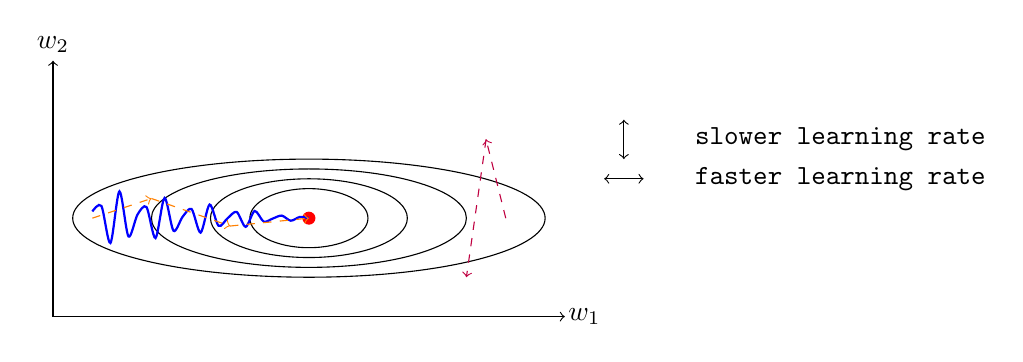
\begin{tikzpicture}
  \draw[->] (-3.25,-2.25) to (-3.25, 1);
  \node at (-3.25, 1.2) {$w_2$};
  \draw[->] (-3.25,-2.25) to (3.25, -2.25);
  \node at (3.5, -2.25) {$w_1$};
  \draw (0,-1) ellipse (3cm and .75cm); 
  \draw (0,-1) ellipse (2cm and .625cm);     
  \draw (0,-1) ellipse (1.25cm and .5cm); 
  \draw (0,-1) ellipse (.75cm and .375cm);
  \node[fill,red,circle,scale=0.5] at (0,-1) {};
  \draw[smooth, domain=-2.75:-.00125, color=blue, thick]
    plot (\x,{1/7*abs(\x)*sin((\x-3)*1250)-1}) {};
  \draw[->,purple,dashed] (2.5,-1) to (2.25, 0);
  \draw[->,purple,dashed] (2.25,0) to (2, -1.75);
  \draw[<->] (4, .25) to (4, -.25);
  \node at (6.75, 0) {\texttt{slower learning rate}};
  \draw[<->] (3.75, -.5) to (4.25, -.5);
  \node at (6.75, -.5) {\texttt{faster learning rate}};
  \draw[->,orange,dashed] (-2.75,-1) to (-2, -.75);
  \draw[->,orange,dashed] (-2, -.75) to (-1, -1.1);
  \draw[->,orange,dashed] (-1, -1.1) to (0, -1);
\end{tikzpicture}
\end{figure}

Notice that initially in this gradient descent trajectory, 
we tend to end up ``on the other side of the 
ellipse'' than intended, this process repeats and 
we end up \emph{oscillating} toward the minimum.
If we try to use a \emph{larger} learning rate, we are likely
to \emph{diverge} (pictured in \color{purple}{purple} 
above\color{black}).
This forces us to use a learning rate that is not too large.
Another way to view this problem, is that on the vertical 
axis, we'd like slower learning, but on the horizontal axis 
we'd like faster learning. This is because the shape of the contours make it easier to ``overshoot'' and end up with a larger cost value when moving up and down relative to left and right.

\paragraph{Momentum} On iteration $t$, we compute $\d W$, $\d b$ on current (mini)-batch. Then, compute
\begin{align*}
V_{\d W} &= \beta V_{\d W} + (1-\beta) \d W \\
V_{\d b} &= \beta V_{\d b} + (1-\beta) \d b
\end{align*}
Our update rule then becomes
\begin{align*}
W &:= W - \alpha V_{\d W} \\
b &:= b - \alpha V_{\d b}
\end{align*}
This has the effect of ``smoothing out'' our steps of gradient descent and in particular it dampens the oscillations that we previously saw. Why is this? Well, if we previously had many up and down oscillations, the average gradient is near zero, whereas on the other hand we are always moving consistently toward the global minimum from left to right and so the weighted average still pulls strongly in this direction; we've plotted this in \color{orange}{orange} \color{black} above.

\paragraph{Intuition} Suppose we have a bowl shaped loss function, and that we plan to roll a ball ``downhill'' toward the global minimum. The terms $\d W$ and $\d b$ describe \emph{acceleration} that we place on the ball, whereas the terms $\beta V_{\d W}$ and $\beta V_{\d b}$ describe \emph{velocity} and in particular wince 
$\beta < 1$ we have a notion of \emph{friction} which prevents
our ball from rolling too fast or out of control.

\paragraph{Hyperparameters} Notice that we've added an additional hyperparameter $\beta$ which controls the exponentially weighted average. The most common value Andrew Ng reports for $\beta$ is 
0.9, which corresponds to averaging over the last $1/(1-.9) = 10$ 
gradients.

\subsection{RMSProp} Momentum was one method of speeding up gradient descent. There's another known as Root Mean Square Prop. On iteration $t$ of (mini) batch gradient descent, we compute the following (where here $\cdot^2$ denotes an element-wise squaring operation.
\begin{align*}   S_{\d W} &= \beta S_{\d W} + (1-\beta) \d W^2 \\ %\hspace{15pt} \tcp{Element-wise square}
  S_{\d b} &= \beta S_{\d b} + (1-\beta) \d b^2 \\ %\hspace{15pt} \tcp{Again, element-wise square}
  W &:= W - \alpha \frac{\d W}{\sqrt{S_{\d W}} + \epsilon} \\
  b &:= b - \alpha \frac{\d b}{\sqrt{S_{\d b}} + \epsilon} \end{align*}

Adam stands for Adaptive Moment Estimation. $\beta_1$ is used to compute the mean of the gradients $\d W$ (first moment) and $\beta_2$ is used to compute the mean of the second moments $\d W^2$.

\paragraph{Intuition}
Notice that it's in the update step where a RMS term appears.
Why does this work? Recall our previous example where in the vertical direction we wanted a smaller learning rate, but for the horizontal direction we wanted a larger learning rate. By incorporating the square of the gradient, we can achieve similar outcomes as with momentum (\emph{dampening gradients that oscillate wildly}).

\paragraph{Implementation Details} In practice, we add some $\epsilon \approx 1e-8$ to the denominator such that we don't divide by something too close to zero (causing our update to blow up).

\subsection{Adam} This is a rare instance of an algorithm that actually works; it works by combining momentum with RMSProp. We first initialize parameters:
\begin{align*}   V_{\d W} = 0, S_{\d W} = 0, V_{\d b} = 0, S_{\d b} = 0 \end{align*}
Then, on iteration $t$, we compute 
$\d W$, $\d b$ using current mini-batch, and then
\begin{align*}   V_{\d W} &= \beta_1 V_{\d W} + (1-\beta_1) \d W \\ 
  V_{\d b} &= \beta_1 V_{\d b} + (1-\beta_1) \d b \\ 
  S_{\d W} &= \beta_2 S_{\d W} + (1-\beta_2) \d W^2 \\
  S_{\d b} &= \beta_2 S_{\d b} + (1-\beta_2) \d b^2 \end{align*}
Typically, we do implement Adam by using $V^{\texttt{corrected}}_{\d W} = \frac{V_{\d W}}{1-\beta_1^t}$ and $V^{\texttt{corrected}}_{\d b} = \frac{V_{\d b}}{1 - \beta_1^t}$ and similarly we have
$S^{\texttt{corrected}}_{\d W} = \frac{S_{\d W}}{1-\beta_2^t}$ and $S^{\texttt{corrected}}_{\d b} = \frac{S_{\d b}}{1-\beta_2^t}$. Then, we perform the updates
\begin{align*}   W &:= W - \alpha \frac{V^{\texttt{corrected}}_{\d W}}{\sqrt{S^{\texttt{corrected}}_{\d W}} + \epsilon} \\
  b &:= b - \alpha \frac{V^{\texttt{corrected}}_{\d b}}{\sqrt{S^{\texttt{corrected}}_{\d b}} + \epsilon} \end{align*}
\paragraph{Hyperparameters}
There are now multiple hyperparameters.
\begin{itemize}   \item $\alpha$ is a hyperparameter that typically needs to be tuned.
\item $\beta_1 \gets 0.9$, i.e. for $\d W$ we average over last ten gradients.
\item $\beta_2 \gets 0.999$, i.e. for $\d W^2$ we average over the last $\frac{1}{1 - 0.999} = 1,000$ gradients.
\item $\epsilon \gets 1e-8$ is typically fixed. \end{itemize}

\subsection{Learning Rate Decay} The idea here is that we take larger steps at first (making steady progress toward the global minimum), but as we approach we start taking smaller steps so as to avoid the problem of dancing around in circles a far region away from the global minimum. To implement learning rate decay, we may choose a heuristic where $\alpha = \frac{1}{1 + \texttt{decay\_rate}*\texttt{epoch\_\#}} \alpha_0$. As a function of the epoch number, this formula (dependent on hyperparameter $\alpha_0$) decays steadily. Another few formulae people try are
\begin{align*}   \alpha &= 0.95^{\texttt{epoch\#}} \cdot \alpha_0 \\
  \alpha &= \frac{k}{\sqrt{\texttt{epoch\#}}} \cdot \alpha_0 \\
  \alpha &= \frac{k}{\sqrt{t}} \cdot \alpha_0 \end{align*}

\subsection{Local Optima} As the field of deep learning has evolved, so has the way we think about local optima. People used to examine low (three) dimensional plots in which it's easy to create many local optima that are significantly worse than the global optimum. In reality in deep learning our parameters $b, W$ live in very high dimensions; in these cases, we are much more likely to run into saddle points as opposed to local optimum. What is a problem in higher dimensions are \emph{plateaus}, and this slows down learning. It is in these cases of plateaus that faster learning algorithms like Adam can really help out.

\end{document}

